\documentclass{article}
\usepackage{geometry}
\geometry{a4paper, margin=1in}
\usepackage{graphicx}
\usepackage[colorlinks=true, linkcolor=blue, citecolor=blue, urlcolor=blue]{hyperref}
\usepackage{listings}
\usepackage{xcolor}
\usepackage{amsmath}
\usepackage{enumitem}
\usepackage{float}

\lstset{
    language=NASM,
    basicstyle=\ttfamily\footnotesize\selectfont, % use the selected monospaced font
    backgroundcolor=\color{white},
    keywordstyle=\color{blue},
    commentstyle=\color{gray},
    stringstyle=\color{red},
    numbers=left,
    numberstyle=\tiny\color{gray},
    stepnumber=1,
    numbersep=10pt,
    frame=single,
    breaklines=true,
    captionpos=b,
    tabsize=4
}

\title{Assignment 1: v04 - Display by VRAM + Inter Segment Move}
\author{
    [Welby Seely] \\
    \texttt{[wseely@emich.edu]}
}
\date{\today}

\begin{document}

    \maketitle
    \section{Intro}\label{sec:intro}
    The v3 version of the bootloader was updated to display (almost) al text from VRAM.

    VGA graphics mode was disabled to enable writing to the memory mapped VRAM region starting at 0xB800.
    Unfortunately, this also disabled drawing the big `W' part of the logo.
    In order to keep it and still write characters manually to VRAM, I would need to manually draw the characters based on a font.
    There should be fonts on the ROM I could use - I might add this to a future version.

    An assembly file with the string `BLOCK DATA, Press Key to Continue \ldots' was added, loaded from logical sector 1 of a.img.
    This sector is then loaded into 0001:7890 so that the `block data' can be read later.
    This string is displayed in lieu of the giant `W'.

    After entering any key, the program clears the screen and switches to display a magenta `\$' and a
    blinking cursor.

    \begin{itemize}
        \item Boot from MBR.
        \item MBR clears screen by VRAM (calls clear\_screen).
        \item MBR loads loaderV04.
        \item loadverV04 displays the `logo' by VRAM.
        \item loaderV04 loads datatimeV04.
        \item loaderV04 calls datatimeV04 as a subroutine, displaying date and time.
        \item loaderV04 returns to MBR.
        \item MBR loads stringV04.asm into memory 0001:7890.
        \item MBR displays the contents of stringV04.asm using BIOS function group 0x10, function 0x13.
        \item MBR waits for a keyboard press.
        \item MBR clears the screen by VRAM.
        \item Then a command prompt `\$' at the top left corner followed by a blinking cursor.
    \end{itemize}

    This fulfills the requiremnts of the assignment.

    \section{Loading from sector 1}\label{sec:reqs}
    int13 function 2 was used to load logical sector 1.

    Equations:
    \begin{itemize}
        \item Physical Sector: \verb|(L % N) + 1|.
        \item Cylinder: \verb|(L / N) / S|.
        \item Head: \verb|(L / N) % S|.
    \end{itemize}
    Where \verb|L| is the logical sector, \verb|T| is the cylinders (tracks) per side, and \verb|S| is the number of sides.

    \begin{itemize}
        \item Sector: \verb|1 % 18 + 1 = 2|
        \item Cylinder: \verb|1 / 18 / 2 = 0|
        \item Head: \verb|1 / 18 % 2 = 0|
    \end{itemize}

    \section{Screenshots}\label{sec:screenshots}
    Screenshots of the splash screen and the prompt screen are provided.

    \begin{figure}[H]  % [H] forces the figure to appear here
        \centering
        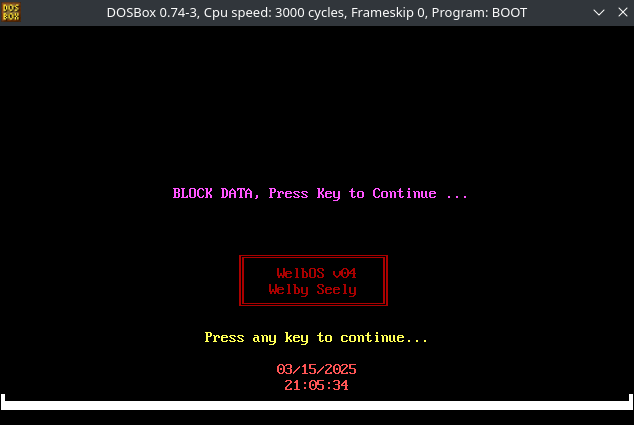
\includegraphics[width=\textwidth]{splash-screen} % Scales image to document width
        \caption{Custom splash screen, complete with block string in the middle}
        \label{fig:1}
    \end{figure}

    \begin{figure}[H]  % Ensures figure appears right here
        \centering
        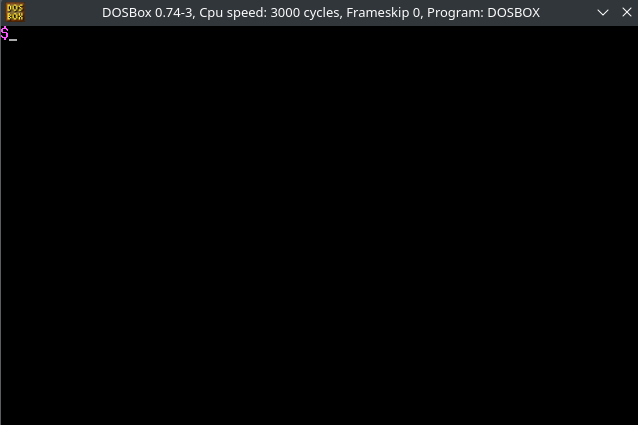
\includegraphics[width=\textwidth]{prompt} % Scales image to document width
        \caption{Prompt with \$ and a blinking cursor}
        \label{fig:2}
    \end{figure}

    \section{Appendix 1: Source Code}\label{sec:appendix_1}
    \begin{lstlisting}[caption={os623V04.asm listing}, captionpos=t]
        bits 16
        BIOS_VIDEO          equ 0x10
        DISPLAY_FUN         equ 0x13

        BIOS_FLOPPY         equ 0x0013
        READ_SECTORS        equ 0x0002

        ; ext code
        MAIN_SEG equ 0x0001
        MAIN_OFF equ 0x2345

        STRING_SEG equ 0x0001
        STRING_OFF equ 0x7890

        MAGENTA_BLACK equ 0x0D

        org 0x7c00
        jmp short start
        nop

        bsOEM       db "WelbOS v03"         ; OEM String

        start:
            ; Inputs: cylinder, sector, head, segment, offset.
            push 1
            push 2
            push 0
            push MAIN_SEG
            push MAIN_OFF

            call 0x:load_sector
            call clear_screen

            call MAIN_SEG:MAIN_OFF
            call print_block_with_bios

            ; restore DS to 0
            push cs
            pop ds

            ; Wait for key press
            mov ah, 0x00
            int 0x16

            call clear_screen

            push MAGENTA_BLACK
            push 1
            push prompt_sym
            push 0
            push 0
            call 0:print

            call set_cursor_pos

            int 20h

        print_block_with_bios:
            ; Inputs: cylinder, sector, head, segment, offset.
            push 0
            push 2
            push 0
            push 0x0001
            push 0x7890

            call 0x:load_sector

            mov bl, MAGENTA_BLACK   ; Attribute
            mov cx, 37              ; length of the string
            mov si, 0x7890          ; address of the string
            mov dh, 10               ; row position
            mov dl, 22               ; column position

            mov ax, 0x01            ; offset
            mov es, ax

            mov  ah, DISPLAY_FUN    ; BIOS display string (function 13h)
            mov  al, 0              ; Write mode = 1 (cursor stays after last char
            mov  bh, 0              ; Video page
            mov  bp, si             ; Put offset in BP (ES:BP points to the string)
            int  BIOS_VIDEO
            ret

        times 0x90 - ($ - $$) db 0

        ; -----------------------------------------------------------------------------
        ; Function: print
        ; Description: Prints a string to the console.
        ; Inputs:
        ;   - [sp+4] Column position to begin writing the string.
        ;   - [sp+6] Row position to begin writing the string.
        ;   - [sp+8] Memory address location of the string.
        ;   - [sp+10] Length of the string.
        ;   - [sp+12] Attribute.
        ; Outputs: None.
        ; Modifies:
        ;   - AX, BX, CX, DX, VGA text buffer section (0xB800)

        ; -----------------------------------------------------------------------------
        print:
            push bp
            mov bp, sp

            ; Set ES to VGA text buffer section (0xB800)
            mov ax, 0xB800
            mov es, ax

            xor ax, ax
            mov al, [bp+8]       ; Load row from stack (byte)
            mov bx, 80           ; 80 columns per row
            mul bx               ; AX = row * 80
            xor dx, dx
            mov dl, [bp+6]       ; Load column from stack (byte)
            add ax, dx           ; AX = (row * 80) + column
            shl ax, 1            ; Multiply by 2 (each char = 2 bytes)
            mov di, ax           ; ES:DI now points to VGA memory location

            ; Set up string parameters
            mov si, [bp+10]      ; String address
            mov cx, [bp+12]      ; String length
            mov ah, [bp+14]      ; Attribute byte (foreground/background)

        .write_loop:
            lodsb                ; Load next character from DS:SI into AL
            stosw                ; Store AX (char + attribute) at ES:DI
            loop .write_loop

            pop bp
            retf 10

        times 0x120 - ($ - $$) db 0

        ; -----------------------------------------------------------------------------
        ; Function: load_sector
        ; Description: Loads a sector into memory
        ; Inputs: cylinder, sector, head, segment, offset.
        ; Outputs: 512 bytes into memory as specified by segment and offset.
        ; Note: Does not currently take into account all 10 bits of the cylinder.
        ; Modifies:
        ;   - AX, BX, CX, DX, EX
        ; Calls:
        ;   - BIOS interrupt 0x13, function 0x02.
        ; -----------------------------------------------------------------------------
        load_sector:
            push bp
            mov bp, sp

            mov bx, [bp + 8]            ; segment (can't move immediate into segment register)
            mov es, bx                  ; segment
            mov bx, [bp + 6]            ; offset
            mov ah, READ_SECTORS        ; function
            mov al, 1                   ; number of sectors to read
            mov ch, [bp + 14]           ; cylinder number (10 bits, upper two bits are 6 and 7 of CL)
            mov cl, [bp + 12]           ; sector number (and upper two of cylinder)
            mov dh, [bp + 10]           ; head (usually same as side)
            mov dl, 0                   ; drive number
            int BIOS_FLOPPY

            pop bp
            retf 10

        set_cursor_pos:
            mov ah, 0x01          ; BIOS Set Cursor Shape function
            mov ch, 0x06          ; Start scan line
            mov cl, 0x07          ; End scan line
            int BIOS_VIDEO        ; BIOS video interrupt

            mov ah, 0x02        ; BIOS function: set cursor position
            mov bh, 0x00        ; Page number (0)
            mov dh, 0x00        ; Row (0)
            mov dl, 0x01        ; Column (1)
            int BIOS_VIDEO
            ret

        clear_screen:
            mov ax, 0xB800      ; Memory-mapped region for text
            mov es, ax
            xor di, di          ; ES:DI = 0xB800:0 (start offset is 0)
            mov ah, 0x07        ; white on black
            mov al, 0x20        ; ASCII space
            mov cx, 2000        ; 80x25 = 2000 characters
            rep stosw           ; Fill screen with spaces and attributes
            ret

        prompt_sym          db "$"

        ; Pad to 512 bytes for an MBR:
        padding times 510 - ($ - $$) db 0

        ; Optional boot signature:
        bootSig db 0x55, 0xAA
    \end{lstlisting}

    \begin{lstlisting}[caption={loaderV04.asm listing}, captionpos=t]
        bits 16
        BIOS_VIDEO          equ 0x10
        DISPLAY_FUN         equ 0x13

        FUN_VIDEO_MODE      equ 0x0000
        VGA_MODE            equ 0x0003

        BIOS_FLOPPY         equ 0x0013
        READ_SECTORS        equ 0x0002

        VGA_DISPLAY_WIDTH   equ 320
        DISPLAY_WIDTH       equ 80
        DISPLAY_HEIGHT      equ 25
        VGA_TXT_DISP_WIDTH  equ 80
        VGA_TXT_DISP_HEIGHT equ 25
        MESSAGE_ROW         equ VGA_TXT_DISP_HEIGHT / 2 + 3
        LINE_ROW_TOP        equ MESSAGE_ROW - 1
        LINE_ROW_NAME       equ MESSAGE_ROW + 1
        LINE_ROW_BOTTOM     equ LINE_ROW_NAME + 1
        LINE_ROW_ANYKEY     equ LINE_ROW_BOTTOM + 2
        TEXT_MODE           equ 0x03
        MAGENTA_BLACK       equ 0x0D
        WHITE_BLACK         equ 0x0F
        RED_BLACK           equ 0x04
        YELLOW_BLACK        equ 0x0E

        BOX_LENGTH          equ 19
        ANYKEY_LENGTH       equ 28
        BITMAP_LENGTH       equ 18
        SHADE_COUNT         equ 9

        SCALING_FACTOR      equ 0x8
        LOGO_START_X        equ (VGA_DISPLAY_WIDTH - (16 * SCALING_FACTOR)) / 2
        LOGO_START_Y        equ (200 - (9 * SCALING_FACTOR)) / 2 -40

        PRINT_SEGMENT       equ 0
        PRINT_OFFSET        equ 0x7c90

        LOAD_SECTOR_SEGMENT equ 0
        LOAD_SECTOR_OFFSET  equ 0x7d00

        DISPLAY_TIME_SEGMENT equ 0x0002
        DISPLAY_TIME_OFFSET  equ 0x3456

        %define CENTER_TXT(len) ((DISPLAY_WIDTH - len) / 2)
        %define CENTER_VGA_TXT(len) ((VGA_TXT_DISP_WIDTH - len) / 2)

        org 0x2345
        main:
            push cs
            pop ds

        hide_cursor:
            mov ah, 0x01          ; BIOS Set Cursor Shape function
            mov ch, 0b00001000    ; Start scan line (set bit 5 to hide cursor)
            mov cl, 0x00          ; End scan line (N/A)
            int BIOS_VIDEO        ; BIOS video interrupt

        show_time:
            push 1
            push 5
            push 0
            push DISPLAY_TIME_SEGMENT
            push DISPLAY_TIME_OFFSET
            call LOAD_SECTOR_SEGMENT:LOAD_SECTOR_OFFSET


        ;    TODO logo can't be drawn in VGA text mode. might work around this later by drawing ASCII directly with font from ROM
        ;    call set_red_gradient_palette
        ;    push LOGO_START_X
        ;    push LOGO_START_Y
        ;    call draw_logo

            push RED_BLACK
            push BOX_LENGTH
            push welbos
            push MESSAGE_ROW
            push CENTER_VGA_TXT(BOX_LENGTH)
            call PRINT_SEGMENT:PRINT_OFFSET

            push RED_BLACK
            push BOX_LENGTH - 1               ; Repeat count
            push CENTER_VGA_TXT(BOX_LENGTH)   ; Column
            push LINE_ROW_TOP                 ; Row
            push topline                      ; Address of 3-tuple
            call draw_line

            push RED_BLACK
            push BOX_LENGTH
            push name
            push LINE_ROW_NAME
            push CENTER_VGA_TXT(BOX_LENGTH)
            call PRINT_SEGMENT:PRINT_OFFSET

            push RED_BLACK
            push BOX_LENGTH - 1       ; Repeat count
            push CENTER_VGA_TXT(BOX_LENGTH)   ; Column
            push LINE_ROW_BOTTOM     ; Row
            push bottomline             ; Address of 3-tuple
            call draw_line

            push YELLOW_BLACK
            push ANYKEY_LENGTH
            push anykey
            push LINE_ROW_ANYKEY
            push CENTER_VGA_TXT(ANYKEY_LENGTH)
            call PRINT_SEGMENT:PRINT_OFFSET

            push WHITE_BLACK
            push VGA_TXT_DISP_WIDTH - 1       ; Repeat count
            push 0   ; Column
            push LINE_ROW_ANYKEY + 4          ; Row
            push blockline                    ; Address of 3-tuple
            call draw_line

            call DISPLAY_TIME_SEGMENT:DISPLAY_TIME_OFFSET

            retf

        draw_logo:
            push bp
            mov bp, sp

            mov ax, [bp + 4]
            mov cx, VGA_DISPLAY_WIDTH
            mul cx
            add ax, [bp + 6]
            mov di, ax

            mov ax, 0xA000     ; memory mapped I/O segment for VGA
            mov es, ax

            mov si, w_bitmap   ; source bitmap start address

            mov dx, 9                  ; logical row that we're calculating
            push SCALING_FACTOR
        draw_rows:
            mov bx, 9
            sub bx, dx                 ; determine color for this row
            mov bl, [row_colors + bx]  ; store row color in BL (or AL, but we’ll need AL soon)
            mov ax, [si]               ; retrieve pixels for this row

            ; Process 16 pixels
            mov cx, 16
        draw_row:
            shl ax, 1          ; Shift left (test MSB of AX)
            jnc skip_column

            push cx
            push ax
            mov cx, SCALING_FACTOR
            mov al, bl
            rep stosb
            pop ax
            pop cx
            jmp next_column
        skip_column:
            add di, SCALING_FACTOR
        next_column:
            loop draw_row

        scale_vertically:
            add di, 320 - 16 * SCALING_FACTOR ; Move to next VGA row
            pop cx
            dec cx
            cmp cx, 0
            jz next_source_row
            push cx
            jmp draw_rows
        next_source_row:
            add si, 2
            dec dx
            jz logo_done
            push SCALING_FACTOR
            jmp draw_rows
        logo_done:
            pop bp
            ret 4

        draw_line:
            push bp
            mov bp, sp

            ;left edge
            push word [bp + 12]
            push 1
            mov si, [bp + 4]
            push si
            mov si, [bp + 6]
            push si
            mov si, [bp + 8]
            push si
            call PRINT_SEGMENT:PRINT_OFFSET

            ; set up middle loop
            mov ax, 1                           ; break when == to cx
        draw_line_middle:
            mov cx, [bp + 10]
            cmp ax, cx
            je draw_line_right
            push ax

            push word [bp + 12]
            push 1
            mov si, [bp + 4]
            inc si
            push si
            mov si, [bp + 6]
            push si
            mov si, [bp + 8]
            add si, ax
            push si
            call PRINT_SEGMENT:PRINT_OFFSET

            pop ax
            inc ax
            jmp draw_line_middle

        draw_line_right:
            push word [bp + 12]
            push 1
            mov si, [bp + 4]
            add si, 2
            push si
            mov si, [bp + 6]
            push si
            add ax, [bp + 8]                    ; rightmostposition
            push ax
            call PRINT_SEGMENT:PRINT_OFFSET

            pop bp
            ret 10

        set_red_gradient_palette:
            mov dx, 0x3C8   ; VGA color index port
            mov al, 32      ; Start setting colors from index 32
            out dx, al
            inc dx          ; Now dx = 0x3C9 (RGB color data port)

            mov cx, 9       ; 9 shades for 9 rows
            mov si, red_shades
        next_color:
            mov al, [si]    ; Load Red intensity
            out dx, al      ; Set Red value
            xor al, al      ; Set Green=0
            out dx, al
            out dx, al      ; Set Blue=0
            inc si
            loop next_color
            ret

        topline             db 0xC9
                            db 0xCD
                            db 0xBB
        bottomline          db 0xC8
                            db 0xCD
                            db 0xBC
        blockline           db 0xDE
                            db 0xDC
                            db 0xDD
        welbos              db 0xBA, `    WelbOS v04   `, 0xBA
        welboslen           equ ($ - welbos)
        name                db 0xBA, `   Welby Seely   `, 0xBA
        namelen             equ ($ - name)
        anykey              db "Press any key to continue..."
        anykeylen           equ ($ - anykey)
        red_shades db 58, 55, 50, 45, 40, 35, 30, 25, 20; Bright to dark red
        ; Row color table, from top to bottom row
        row_colors db 32, 33, 34, 35, 36, 37, 38, 39, 40  ; Use only custom red shades
        w_bitmap db 02h, 80h
                 db 02h, 80h
                 db 04h, 40h
                 db 04h, 40h
                 db 08h, 21h
                 db 88h, 22h
                 db 50h, 14h
                 db 50h, 14h
                 db 20h, 08h

    \end{lstlisting}
    \begin{lstlisting}[caption={datetimeV04.asm listing}, captionpos=t]
        PRINT_SEGMENT       equ 0
        PRINT_OFFSET        equ 0x7c90

        VGA_TXT_DISP_HEIGHT equ 25
        VGA_TXT_DISP_WIDTH  equ 80

        MESSAGE_ROW         equ VGA_TXT_DISP_HEIGHT / 2 + 3
        LINE_ROW_TOP        equ MESSAGE_ROW - 1
        LINE_ROW_NAME       equ MESSAGE_ROW + 1
        LINE_ROW_BOTTOM     equ LINE_ROW_NAME + 1
        LINE_ROW_ANYKEY     equ LINE_ROW_BOTTOM + 2
        LIGHT_RED           equ 0x0C

        %macro makedt 4
            mov bh,%1 			;dh/dl/chcl
            shr bh,4
            add bh,30h 			;add 30h to convert to ascii
            mov [%2 + %3],bh
            mov bh,%1
            and bh,0fh
            add bh,30h
            mov [%2 + %4],bh
        %endmacro

        %define CENTER_VGA_TXT(len) ((VGA_TXT_DISP_WIDTH - len) / 2)

        bit16
        org 0x3456

            push ds
            push cs
            pop ds

            mov ah,04h	 ;function 04h (get RTC date)
            int 1Ah		;BIOS Interrupt 1Ah (Read Real Time Clock)

            makedt dh, dtfld, 0, 1  ; month
            makedt dl, dtfld, 3, 4  ; day
            makedt ch, dtfld, 6, 7  ; century
            makedt cl, dtfld, 8, 9  ; year

            mov ah,02h
            int 1Ah

            makedt ch, tmfld, 0, 1  ; hours
            makedt cl, tmfld, 3, 4  ; minutes
            makedt dh, tmfld, 6, 7  ; seconds

            push LIGHT_RED
            push 10
            push dtfld
            push LINE_ROW_ANYKEY + 2
            push CENTER_VGA_TXT(10)
            call PRINT_SEGMENT:PRINT_OFFSET

            push LIGHT_RED
            push 8
            push tmfld
            push LINE_ROW_ANYKEY + 3
            push CENTER_VGA_TXT(8)
            call PRINT_SEGMENT:PRINT_OFFSET

            pop ds
            retf

        dtfld: db '00/00/0000'
        tmfld: db '00:00:00'
    \end{lstlisting}

    \begin{lstlisting}[caption={stringV04.asm listing}, captionpos=t]
        db 'BLOCK DATA, Press Key to Continue ...'
    \end{lstlisting}
    \end{document}
